\documentclass[titlepage,a4paper,twoside,9pt]{article}
\usepackage{prettyref}
\usepackage{hyperref}
\usepackage{graphicx}
\usepackage{multicol}
\usepackage{xcolor}
\usepackage{caption}
\usepackage{subcaption}
\usepackage{setspace}
\usepackage{xspace}
\usepackage[left=3cm,right=2cm,top=3cm,bottom=5cm,includeheadfoot]{geometry}

\onehalfspacing 

\title{MarVis-Graph User Manual}
\author{Manuel Landesfeind}

\newcommand{\mg}{Mar\-Vis--Graph\xspace}
\newcommand{\organism}[1]{\textit{#1}\xspace}
\newcommand{\ath}{\organism{A. thaliana}}
\newcommand{\excel}{Microsoft\textsuperscript{\textregistered} Excel\textsuperscript{\textregistered}\xspace}
\newcommand{\mgap}{\ensuremath{g_\text{max}}}
\newcommand{\mcofactor}{\ensuremath{c_\text{cofactor}}}
\newcommand{\rwr}{\textit{random walk with restart}}
\newcommand{\name}[1]{\textit{#1}}
\newcommand{\aclink}[2][ARA]{\url{http://pmn.plantcyc.org/#1/NEW-IMAGE?&object=#2}, accessed May 14th 2013}
\newcommand{\mm}{metabolite marker\xspace}
\newcommand{\mms}{metabolite markers\xspace}

\newrefformat{fig}{Figure \ref{#1} ``\nameref{#1}''}
\newrefformat{tab}{Table \ref{#1} ``\nameref{#1}''}
\newrefformat{sec}{Section \ref{#1} ``\nameref{#1}''}
\newrefformat{ssec}{Subsection \ref{#1} ``\nameref{#1}''}
\newrefformat{sssec}{Subsection \ref{#1} ``\nameref{#1}''}
\newcommand{\pref}[1]{\prettyref{#1}}

\newcommand{\menu}[3]{``#1'' $\rightarrow$ ``#2'' (Shortkey: Ctrl+#3)}

\usepackage{arev}

\begin{document}
\maketitle

\section{Introduction}


\section{Installation}

A \mg installer is available as supplemental material to our paper
\cite{landesfeind2013marvisgraph} or may be downloaded at:
\url{http://marvis.gobics.de}
To install \mg, follow the instructions of the installer. After successfull
installation, \mg can be started via your applications menu.

\subsection{Prerequirements} For the installer and for \mg itself, the Java
Runtime Environment v1.7 (JRE7) or higher is required. JRE7 can be downloaded
(if it is not already installed) free of charge at \url{http://www.java.com}

\mg has been developed on an 64-bit system with Ubuntu Linux 12.10 ``Quantal Quetzal''
\footnote{\url{http://www.ubuntu.com}} using the Netbeans IDE 7
\footnote{\url{https://netbeans.org/}}. Additionally, \mg has been used under
Windows 7\footnote{\url{http://windows.microsoft.com}}. It has \textbf{not}
been tested under Mac OSX and is therefore not supported on Mac. 

\section{User Interface}
\begin{figure}
	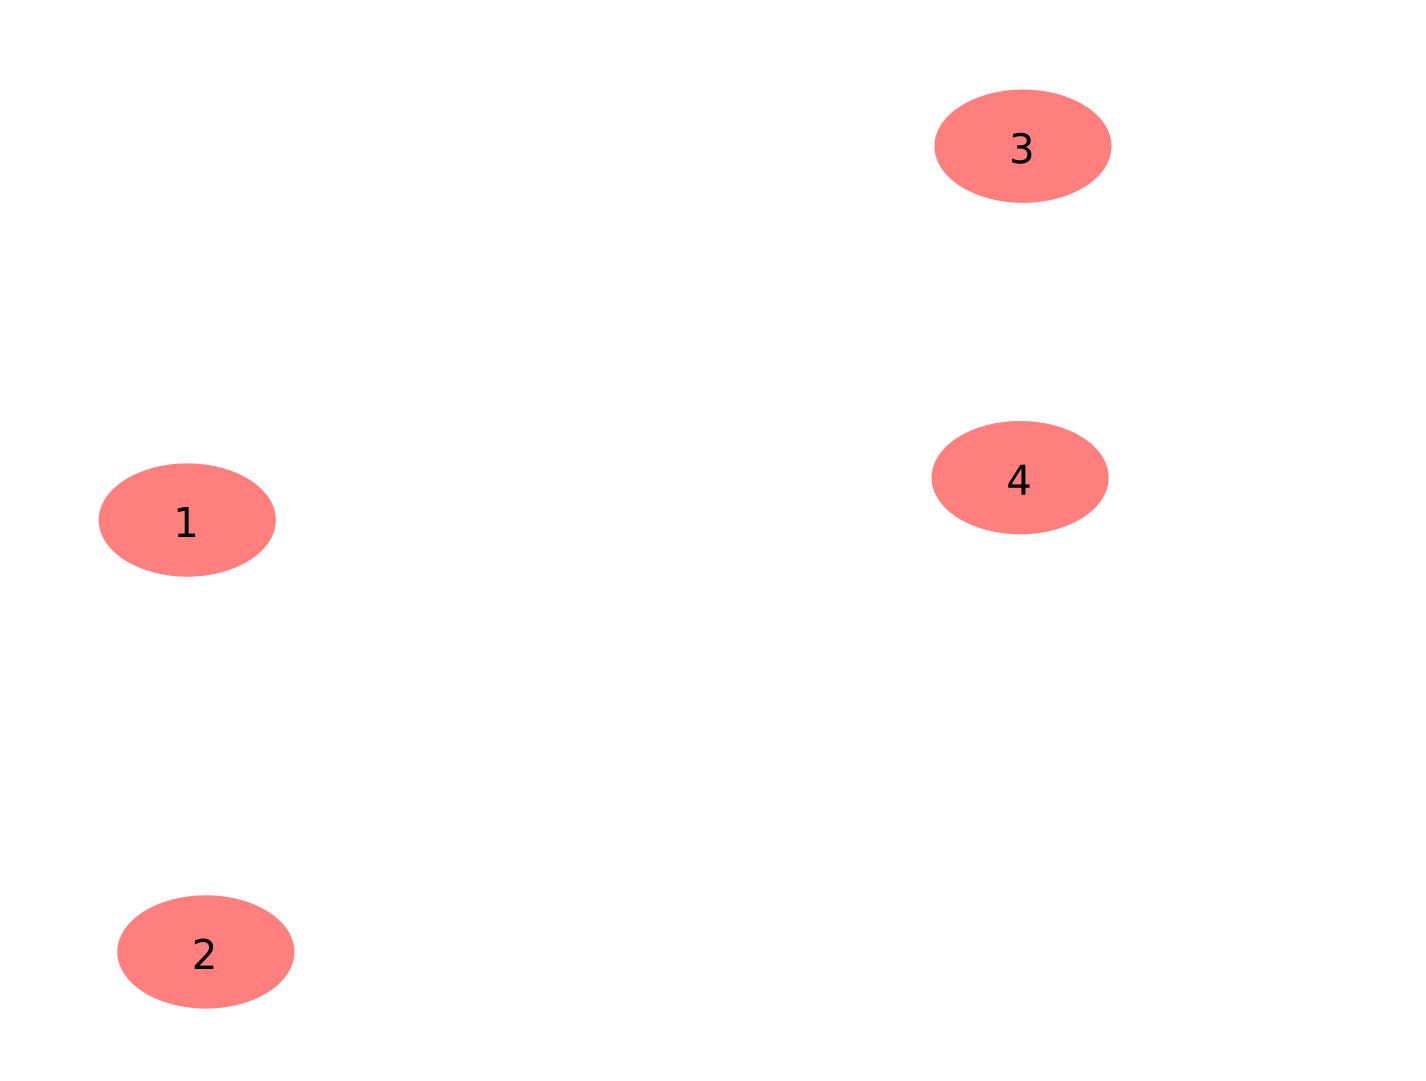
\includegraphics[width=\textwidth]{images/main.pdf}
	\caption[\mg main window]{\mg main window: 1) list of the main network and
		sub--networks sorted according to the selected scoring method. 2)
		Basic information about the contents of the selected network. 3) Setup
		the visualization of the network. 4) Visualization of the network.
		\label{fig:main}}
\end{figure}
The \mg main window, shown in \pref{fig:main}, displays informations in
different areas.

\subsection{Network/Sub--Network list}

On the left side a tree structure displays the different networks calculated.
The root of the tree, i.e. the upper node, is the main network where all
database and experimental data has been integrated. The networks below are
calculated sub--network. When sub--networks are calculated, this tree changes:
first the old sub--networks are irrevocably removed and afterwards the newly
calculated networks are added.

\paragraph{Sorting} The sub--networks can be sorted according to different
scoring methods (see \pref{sssec:scoring}). On top of the sub--network tree a
box is displayed providing accession to the different scoring methods. On
selection of a different method the scores are recalculated and the tree view
is updated.

\section{Using \mg}

\subsection{Building a new network from the database
sources}\label{ssec:newnetwork}

Before experimental data can be imported into \mg, a metabolic network model
has to be created. \mg currently supports the KEGG and BioCyc database
collections.

While the BioCyc database collection contains more organism--specific networks
from which some are manually curated, the usage of KEGG is preferred as the
download can be done fully automatically.

\begin{figure}
	\begin{subfigure}[b]{0.45\textwidth}
		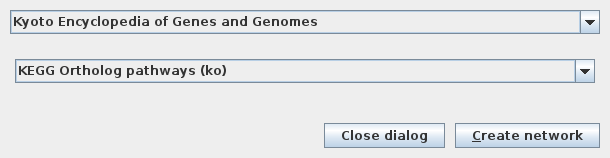
\includegraphics[width=\textwidth]{images/create_network_kegg.png}
		\caption{Create network from KEGG\label{fig:newnetwork_kegg}}
	\end{subfigure}
	\begin{subfigure}[b]{0.45\textwidth}
		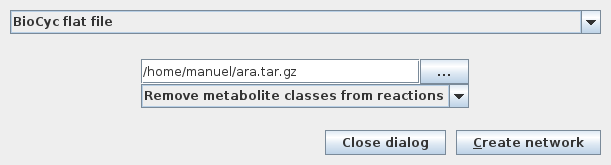
\includegraphics[width=\textwidth]{images/create_network_biocyc.png}
		\caption{Create network from Biocyc\label{fig:newnetwork_biocyc}}
	\end{subfigure}

	\caption[Create new network]{Create a new metabolic network model.
		Depending on the selection between KEGG and Biocyc the options of the
	dialog change. The options are described in \pref{ssec:newnetwork}
	\label{fig:newnetwork}}
\end{figure}

\paragraph{KEGG: Kyoto Encyclopedia of Genes and Genomes}
\cite{kanehisa2010kegg,kanehisa2000kegg} Creating a new metabolic network
model from the KEGG database is done via the KEGG REST
API\footnote{\url{http://www.kegg.jp/kegg/rest}}. 

When KEGG is selected as source in the upper drop--down menu (see
\pref{fig:newnetwork_kegg}), a request is
send to the KEGG webservice to fetch a full list of organisms available.
Afterwards, the organism under research can be selected in the lower
drop--down menu. If no such organism is available the ``KEGG Ortholog Pathways
(KO)'' may be used. This metabolic network contains all reactions in KEGG
(reference network).

Please note that the transmission of data from the KEGG webservice is slow and
the creation may take a while. However, a progressbar will
pop up and display the progress.

\paragraph{BioCyc database collection} \cite{caspi2008metacyc,
caspi2010metacyc,caspi2012metacyc} To create a metabolic network model from
a BioCyc database, the first step is the manual download of the database
because of the license requirements from BioCyc.
After a request for the ``Data File License''
\footnote{\url{http://biocyc.org/download.shtml}} one will receive an email
containing a link to the download page. Here, all individual databases are
listed and the required database can be downloaded as ``tarball'' (file
extension: ``.tar.gz'' or ``.tgz'').
In the \mg dialog for network creation using the BioCyc flat files (see
\pref{fig:newnetwork_biocyc}), the priviously downloaded file has to be selected. 

The import of BioCyc databases requires a specific option determining the
handling of metabolite classes in reactions:
\begin{description}
	\item[Remove metabolite classes from reactions]
		All classes are removed from the reactions resulting in a more sparse
		network. Therefore, connections between reactions may be missed.
	\item[Use metabolite classes as metabolites]
		Each class is assumed to be a metabolite and used stricly. Unfortunately, the classes have no
		monoisotopic mass and annotating them with experimental evidence is hard.
	\item[Substitute classes with metabolites]
		Each class is substituted by the metabolites it represents. This
		results in reactions with a lot of substrates and products.
	\item[Build reactions for each variant]
		For each reaction with class as reactant, all possible variants of the
		reaction are added as single reaction to the network.
		Therefore, metabolites may be associated with a lot of reaction which
		may later interfere with the hub--metabolite threshold (see
		\pref{ssec:calculate}).
\end{description}
Every option has its advantages and disadvantages and it depends on the
hypothesis to be investigated which representation of classes may be the best.
If in doubt, the proposed strategy is the removal of all metabolite clases
form the reactions.

\subsection{Saving and loading a metabolic network}\label{ssec:saveload}

Metabolic network models can be stored and loaded from \mg using a simple XML
file format. To reduce the required space on the harddisk, the XML may be
compressed utilizing the Lembel--Ziv--77 algorithm (gzip).

After creation of a metabolic network it can be saved to harddisk
via the menu ``File'' $\rightarrow$ ``Save network'' (shortkey Crtl + S). 
After selecting a destination and filename, \mg write all data from the
network into that file. 

Similarily, a network can be (re-)loaded into \mg via the menu ``File''
$\rightarrow$ ``Load network'' (shortkey Crtl + L). After selecting a valid
\mg network file the network is imported and set as root network in the
network tree. Hereby, a previously loaded or created network will be removed
without notification.

\subsection{Importing experimental data}\label{ssec:import_experimental_data}

When a metabolic network model is loaded or created in \mg, experimental
data can be added. \mg loads them from tabular data files. Currently, the
following file formats are supported:
\begin{description}
	\item[Comma--Separated--Values (*.csv)\footnote{\url{http://en.wikipedia.org/wiki/Comma-separated_values}}]
		This text file format is the simplest. On import, several additional
		parameters need to be given, e.g. the cell separator and quote
		character (see \pref{fig:dialog_import_1}).
	\item[Microsoft Excel (*.xls, *.xlsx)\footnote{\url{http://office.microsoft.com}}]
		\mg can directly import data from the Excel spreadsheet file format.
		On import, the sheet to be imported needs to be specified (see
		\pref{fig:dialog_import_2}).
\end{description}

\begin{figure}
	\begin{subfigure}{\textwidth}
		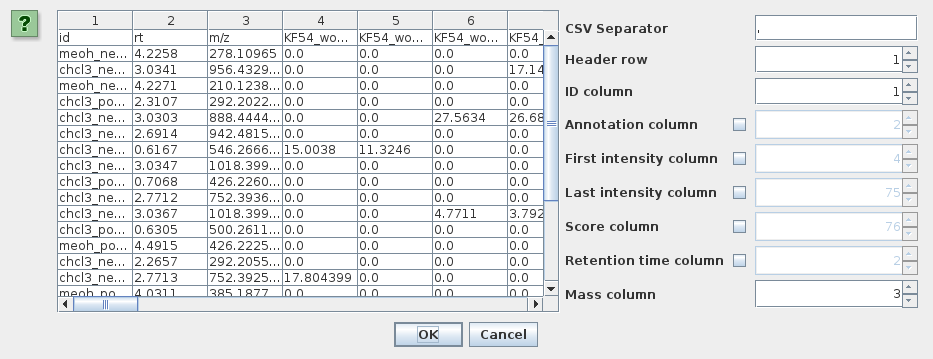
\includegraphics[width=\textwidth]{images/dialog_import.png}
		\caption{Import metabolite markers from a CSV file.\label{fig:dialog_import_1}}
	\end{subfigure}
	
	\vfill

	\begin{subfigure}{\textwidth}
		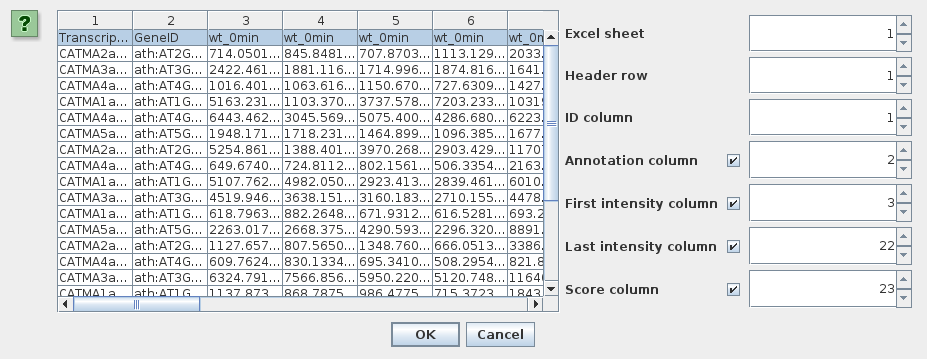
\includegraphics[width=\textwidth]{images/dialog_import2.png}
		\caption{Import transcriptomics markers from an Excel file.\label{fig:dialog_import_2}}
	\end{subfigure}
	\caption[Experimental data import]{The experimental data import dialog
		shows a preview of the data to be imported on the left side and
		specific options on the right side. This dialog is from CSV import
		while during an import from Excel files, instead of a ''Separator``
		the sheet to be imported has to be specified. The options are
	explained in \pref{ssec:import_experimental_data}}
	\label{fig:import_dialog}
\end{figure}

After selection of the file to import, options for the import have to be set.
The set of general options is:
\begin{description}
	\item[CSV Separator] (only on CSV import) Specifies the character that is
		used to split a line into its different cells (see
		\pref{fig:dialog_import_1}). When changed, the
		preview on the left side is updated automatically.
	\item[Excel sheet] (only on Excel import) Specifies the sheet from which
		the data is imported (see \pref{fig:dialog_import_2}). When changed, the
		preview on the left side is updated automatically.
	\item[Header row] (mandatory) specifies the row that contains the head of the table,
		i.e. the description of the columns. In \pref{fig:import_dialog} the
		header row is 1.
	\item[ID column] (mandatory) is the column containing the IDs of the experimental
		marker. Please note that \mg distinquishes between \mms and transcript
		markers but within this groups, all experimental need to have distinct
		IDs. Otherwise, the previous experimental marker will be overwritten.
	\item[Annotation column] (optional) A column containing the annotation of the
		experimental marker. For \mms, this has to be the ID of the compound
		while for transcript markers, this needs to be the ID of the
		corresponding gene. For each experimental marker only one annotation
		is supported.
	\item[First intensity column] (optional) The first column that contains
		abundance/intensity information.
	\item[Last intensity column] (optional) The last column that contains
		abundance/intensity information.
	\item[Score column] (optional) This column contains the score for each experimental
		marker. If not given, a default score of $1$ is assumed for all
		experimental marker.
\end{description}

\subsubsection{Metabolite Marker}

For \mms import more columns can be specified.
\begin{description}
	\item[Retention time column] (optional) The column containing the
		retention time measured by a gas or liquid chromatography. This data
		is not used but displayed.
	\item[Mass column] (mandatory) Specifies the column containing the
		measured masses (corrected mass--to--charge ratios) or the
		experimental marker. This mass is used to relate \mms
		with their metabolites if no annotation is given separately.
\end{description}

\subsection{Calculating sub--networks}\label{ssec:calculate}

To analyse the metabolic network, sub--networks need to be identified. The
menu item \menu{File}{Calculate networks}{C} becomes available when a
metabolic network is loaded. 

On activation, a dialog requests for the method of extraction and the specific
parameters. Currently, two methods are supported:

\paragraph{Pathways} Here, \mg simply extracts all reactions per pathway and
creates a new sub--network from them. 

\paragraph{Random Walk Based} This is the proposed method for the analysis
using \mg as described in \cite{landesfeind2013marvisgraph}. The scores of the
experimental markers is equally distributed to the reactions associated with
an experimental marker. The accumulated scores of the reactions are used as
initial scores to the \rwr algorithm as described in \cite{glaab2012nsea}
using the user--defined ``Restart probability'' (see
\pref{fig:dialog_calculate}) ignoring metabolites that are connected to more
than reactions than specified by the ``Hub metabolite threshold''.
Finally, \mg removes all reactions with a score lower than the ``Score
threshold''. Here, the metabolic network is decomposed into different
components from which each is a resulting sub--network.
These are displayed in the main windows network tree (see \pref{fig:main}).

\begin{figure}
	\begin{center}
		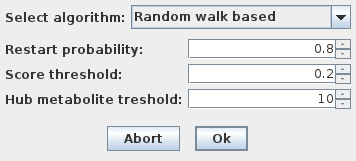
\includegraphics[scale=0.7]{images/dialog_calculate.png}
	\end{center}
	\caption[Calculate sub--networks]{For the calculation of the
		sub--networks a method needs to be choosen and specific parameters can
	be set to tune the method depending on the input data.}
	\label{fig:dialog_calculate}
\end{figure}


\subsubsection{Scoring sub--networks}\label{sssec:scoring}

The sub--networks identified are presented as ranked list. The ranking method
can be changed using the box above the network list in the main window.

\begin{description}
	\item[Size] The score equals the number of reactions within the
		sub--network.
	\item[Sum of weights] Sums up the weights of the \mms and transcripts
		makers per sub--network.
	\item[Diameter]\footnote{\url{http://en.wikipedia.org/wiki/Distance\_\%28graph\_theory\%29}}
		Calculates the shortest paths between all reactions and uses the
		length of the longest path as score.
\end{description}

\subsubsection{Perform a random permutation test}

The ranking of the identified sub--networks can be evaluated using a random
permutation test via the menu \menu{File}{Permutation Test}{P}. This menu item
is only available when sub--networks have been identified. 

On selection, a dialog requests for the number of permutations to be performed
and the number of CPUs that may be used in parallel to speed up the
calculation process. Even with parallel calculation, this may take a long
time for a high number of permutations.

Finally, the results are displayed as table containing the sub--network name,
its score, and the family wise error rate (FWER) and false discovery rate
(FDR) during the permutation test. The results can be exported into tabular
data files (CSV or \excel).

\subsection{Visualizing and inspecting networks}

The sub--networks are visualized using the Java Universal Network/Graph
Framework 2 (JUNG \footnote{\url{http://jung.sourceforge.net}}). After
selection of a sub--network from the list of networks (marked by ``1'' in
\pref{fig:main}), basic statistics of the sub--network contents are shown
below (marked by ``2''). With a click on the ``Draw network'' button, the
network is visualized in the right side of the main window. Depending on the
size of the network the calculation of the layout may take some time.

\begin{figure}
	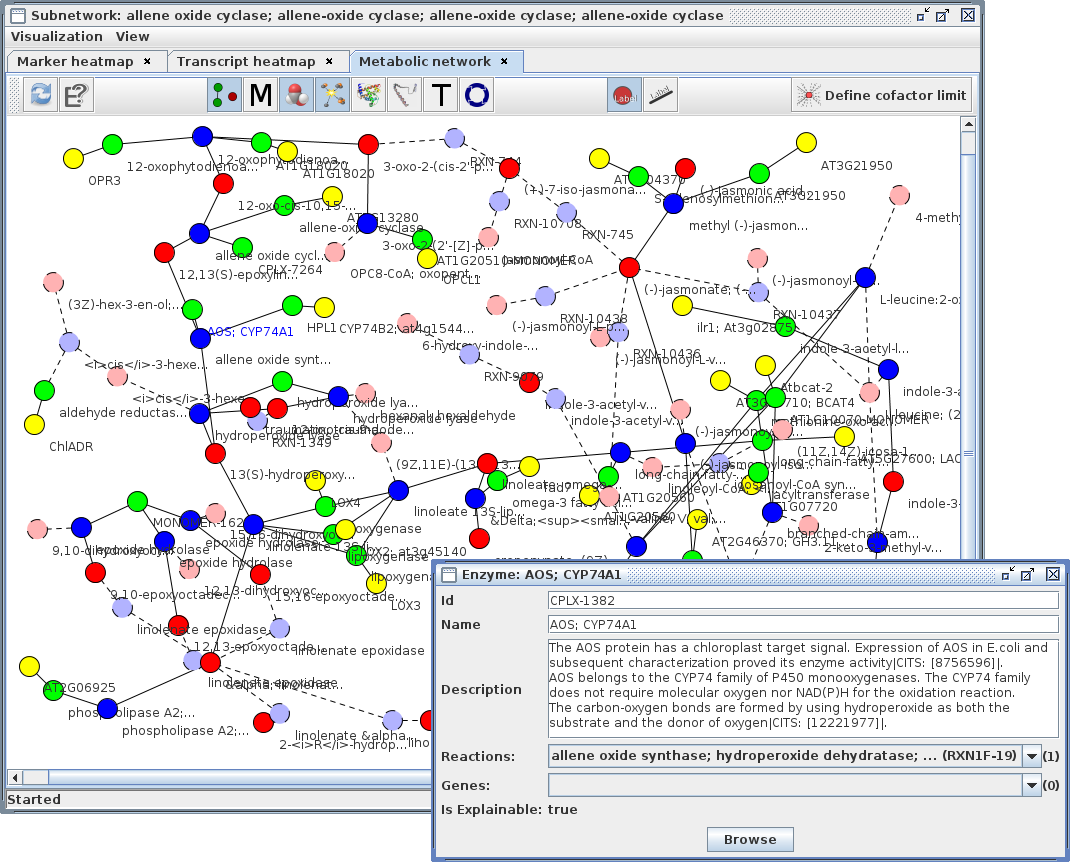
\includegraphics[width=\textwidth]{images/network_visualization.png}
	\caption[Network visualization window]{Separate windows with the \mg main
		window display the identified sub--networks. The layout may be redrawn
		or changed using the short buttons. Also heatmaps of the experimental
		markers are available.}
	\label{fig:network_visualization}
\end{figure}

A visualization of the network is displayed as separate windo within the \mg
main window (see \pref{fig:network_visualization}). The colored nodes in the
visualiation represent the different entities of the network:
\begin{multicols}{2}
	{\bf
	\begin{itemize}
		\item \textcolor{gray}{\mms: gray}
		\item \textcolor{pink}{transcript markers: pink}
		\item \textcolor{red}{Metabolites: red}
		\item \textcolor{blue}{Reactions: blues}
		\item \textcolor{green}{Enzymes: green}
		\item \textcolor{yellow}{Genes: yellow}
		\item \textcolor{cyan}{Pathways: cyan}
	\end{itemize}}
\end{multicols}

The computer mouse may be used to adjust the visualization:
\begin{itemize}
	\item Zooming\\
		The visualization may be zoomed in and out via the mouse wheel.
	\item Panning\\
		To pan the complete network, a right--click on the visualization while
		moving the mouse is used.
	\item Selecting a group of nodes\\
		Keeping the left mouse button clicked while moving the mouse selects a
		group of nodes. A rectangle showing the area of selecting and
		afterwards, the labels of the selected nodes are displayed in
		\textcolor{blue}{blue}.
	\item Moving nodes\\
		All nodes in the networks can be moved by clicking on them and
		dragging them to a new location. The nodes can be either moved
		individually or as group when selected before.
	\item Node information\\
		A double left--click on a node opens a window showing additional
		information, e.g. description or abundance/intensity
		profile.
\end{itemize}
	

\subsubsection{Chancing the layout}\label{sssec:layout}

The visualization can be adapted by hiding specific types of nodes. For
example, when only \mms are imported the genes and enzymes may be less
interesting. A click on the ``E?'' button (see \pref{fig:network_visualization})
opens a dialog to specify the types to display.
\begin{itemize}
	\item \textbf{None}\\
		No nodes of this kind are displayed.
	\item \textbf{With marker}\\
		Nodes are only displayed when experimental marker are somehow
		associated with them.
	\item \textbf{All} (default)\\
		All nodes are displayed.
\end{itemize}

Additionally a ``hub metabolite threshold'' can be used to hide nodes
associated with many nodes. These are often co--factors as water, ATP, or
NAD(H)/NADP(H).

\begin{figure}
	\begin{center}
		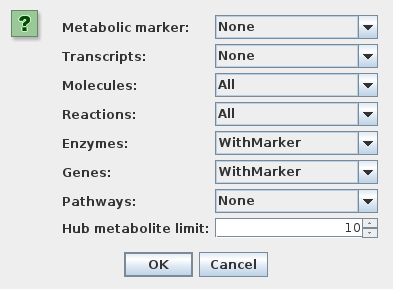
\includegraphics[scale=0.5]{images/network_visualization_types.png}
	\end{center}
	\caption[Settings for visualization]{Settings for network visualization
		allows to show/hide nodes depending on their experimental evidence or
		completely. The settings are explained in \pref{sssec:layout}.}
\end{figure}

\subsubsection{Exporting the graphic}

A right--click on the visualization opens a menu that includes a menu item for
graphic export. Here, only an export into the Scalable Vector Graphics format
(*.svg)\footnote{\url{http://de.wikipedia.org/wiki/Scalable_Vector_Graphics}}.

\section{Contact}
\mg has been developed at the Department for Bioinformatics at the
Georg--August--University in G\"ottingen (Germany).
If you have question or suggestions regarding the software, please write to
\href{mailto:marvis@gobics.de}{marvis@gobics.de}.

\subsection{License}
\mg is released under the terms of the GNU General Public License
v3\footnote{\url{http://www.gnu.org/licenses/gpl-3.0.txt}}> 

\begin{quote}\mg is free software: you can redistribute it and/or modify
    it under the terms of the GNU General Public License as published by
    the Free Software Foundation, either version 3 of the License, or
    (at your option) any later version.

    This program is distributed in the hope that it will be useful,
    but WITHOUT ANY WARRANTY; without even the implied warranty of
    MERCHANTABILITY or FITNESS FOR A PARTICULAR PURPOSE.  See the
    GNU General Public License for more details.

    You should have received a copy of the GNU General Public License
	along with this program.  If not, see \url{http://www.gnu.org/licenses}.
\end{quote}

Usage of \mg is free of charge in academic research. Commercial users please
contact \href{mailto:marvis@gobics.de}{marvis@gobics.de} for license
information.

\subsection{Cite}

If you use \mg in your research, please cite:
\cite{landesfeind2013marvisgraph}


\bibliographystyle{plain}
\bibliography{../../promotion/Library}

\end{document}

